%%%%%%%%%%%%%%%%%%%%%%%%%%%%%%%%%%%%%%%%%%%%%%
% curso git y Github para ciencia reproducible
% 2. Colaborando
%
% Barcelona, 10-12 Febrero 2025
%
% Urtzi Enriquez-Urzelai
%%%%%%%%%%%%%%%%%%%%%%%%%%%%%%%%%%%%%%%%%%%%%%


% Inbuilt themes in beamer
\documentclass{beamer}

% additional packages:
\usepackage{minted}
\usepackage{svg}
\usepackage{caption}
\usepackage{fontawesome}

% Theme choice:
\usetheme{Madrid}
\makeatother
\setbeamertemplate{footline}
{
\leavevmode%
  \hbox{%
  \begin{beamercolorbox}[wd=.2\paperwidth,ht=2.25ex,dp=1.1ex,center]{section in head/foot}%
    \usebeamerfont{section in head/foot}\insertsection
  \end{beamercolorbox}%
  \begin{beamercolorbox}[wd=.8\paperwidth,ht=2.25ex,dp=1.1ex,center]{title in head/foot}%
    \usebeamerfont{title in head/foot}\insertshorttitle\hspace*{24em}
    \insertframenumber{} / \inserttotalframenumber\hspace*{1ex}
  \end{beamercolorbox}}%
}
\makeatletter
\setbeamertemplate{navigation symbols}{}
\setbeamertemplate{caption}[numbered]
\captionsetup[figure]{font=tiny}

% Title page details: 
\section{}
\title{\texttt{git} y \texttt{GitHub} para ciencia reproducible}
\subtitle{2. Colaborando}
\author{Urtzi Enriquez-Urzelai\inst{1}}
\institute{ 
    \inst{1} Institute of Vertebrate Biology,
    \newline  
    Czech Academy of Sciences 
    \newline \newline
    \faGithub \hspace*{0.2ex} \href{https://github.com/urtzienriquez}{\color{blue}{GitHub}}
    \hspace*{0.5ex} \faGlobe \hspace*{0.2ex} \href{https://urtzienriquez.github.io/}{\color{blue}{webpage}}
    }
\date{\today}
\logo{
\includegraphics[height=1.0cm,keepaspectratio]{../1_introduccion/images/IVB-logo-en-color-big.png}}


\begin{document}

% Title page frame
\begin{frame}
    \titlepage 
\end{frame}

% Remove logo from the next slides
\logo{}

% Outline frame
\begin{frame}{Contenido}
    \tableofcontents
\end{frame}


%%% List of frames

% Conceptos básicos
\section{Esenciales}

\begin{frame}[fragile]{Conceptos básicos}
    Para trabajar en equipo es necesario conocer algunos
    conceptos básicos. \\~\\ \pause
    Ya sabemos:
    \setbeamercovered{transparent}
    \begin{columns}
        % Column 1
        \begin{column}{0.4\textwidth}
            \begin{itemize}
                \setlength\itemsep{1.2em}
                \item<2-> Crear un repositorio
                \item<3-> Añadir cambios
                \item<4-> Hacer un "commit" (i.e. una captura) de los cambios
                \item<5-> Volcar los cambios al repositorio remoto
            \end{itemize}
        \end{column}
        % Column 2    
        \begin{column}{0.42\textwidth}
            \begin{exampleblock}{}<2->
                \scriptsize
                \begin{minted}[autogobble]{bash}
                    # Iniciar un repositorio
                    $ git init
                \end{minted}
            \end{exampleblock}
            \begin{exampleblock}{}<3->
                \scriptsize
                \begin{minted}[autogobble]{bash}
                    # Añadir cambios
                    $ git add .
                \end{minted}
            \end{exampleblock}
            \begin{exampleblock}{}<4->
                \scriptsize
                \begin{minted}[autogobble]{bash}
                    # Capturas "estado"
                    $ git commit -am "some cool commit"
                \end{minted}
            \end{exampleblock}
            \begin{exampleblock}{}<5->
                \scriptsize
                \begin{minted}[autogobble]{bash}
                    # Subir a repositorio remoto
                    $ git push
                \end{minted}
            \end{exampleblock}
        \end{column}
    \end{columns}
    \setbeamercovered{invisible}
\end{frame}

% Clone
\section{\texttt{clone}}

\begin{frame}[fragile]{\texttt{clone}}
    Clonar un repositorio suele ser muchas veces
    el primer paso para trabajar en un 
    repositorio que ya ha sido depositado online. \\~\\
    \begin{exampleblock}{código}
        \scriptsize
        \begin{minted}[autogobble]{bash}
            # navegar a la carpeta donde guardaremos el repositorio
            $ cd path/to/store/the/repo
                    
            # clonar el repositorio
            $ git clone https://github.com/urtzienriquez/test
        \end{minted}
    \end{exampleblock}
\end{frame}

% Pull
\section{\texttt{pull}, \texttt{fetch} y \texttt{merge}}

\begin{frame}[fragile]{\texttt{pull}, \texttt{fetch} y \texttt{merge}}
    \begin{columns}[T]
        % Column 2    
        \begin{column}{0.5\textwidth}
            Una operación habitual cuando más de una
            persona trabaja en un mismo repositorio es,
            \texttt{pull}. \\~\\
            \texttt{pull} nos permite sincronizar 
            localmente los cambios que (otrxs colaboradorxs) 
            han volcado en el repositorio remoto. \\~\\
            \texttt{pull} es equivalente a hacer \texttt{fetch}
            seguido de \texttt{merge}. 
        \end{column}
        % Column 1
        \begin{column}{0.4\textwidth}
            \begin{exampleblock}{código}
                \scriptsize
                \begin{minted}[autogobble]{bash}
                    # sincronizar localmente
                    $ git pull

                    # equivalente a 
                    $ git fetch && git merge
                \end{minted}
            \end{exampleblock}
        \end{column}
    \end{columns}
\end{frame}

% Ramas
\section{Trabajando con ramas}
\begin{frame}[fragile]{Trabajando con ramas}
    Trabajar con \textbf{ramas} es esencial para
    evitar pisarnos los pies. \\~\\ %\pause
    De esta manera sabemos que el código que
    estamos modificando no interfiere con las
    posibles modificaciones de un colaborador. \\~\\
    \begin{columns}
        % Column 2    
        \begin{column}{0.3\textwidth}
            \begin{figure}
                \centering
                \includesvg[width=0.7\textwidth,keepaspectratio]{../1_introduccion/images/func_git_3.svg}
                \caption{Nueva rama.}
            \end{figure}
        \end{column}
        % Column 1
        \begin{column}{0.6\textwidth}
            \begin{exampleblock}{código}
                \scriptsize
                \begin{minted}[autogobble]{bash}
                    # consultar qué ramas tenemos
                    $ git branch

                    # crear una nueva rama
                    $ git branch -c new_analysis

                    # movernos a la nueva rama
                    $ git switch new_analysis
                \end{minted}
            \end{exampleblock}
        \end{column}
    \end{columns}
\end{frame}

% cómo contribuir
\section{Contribuyendo}
\begin{frame}{Cómo contribuir. \texttt{pull request}}
    La manera más respetuosa de contribuir es mediante \texttt{pull request}s. \\~\\ %\pause
    Tanto si estamos trabajando en una rama o en un repositorio
    bifurcado (\texttt{fork}).
    \begin{figure}
        \centering
        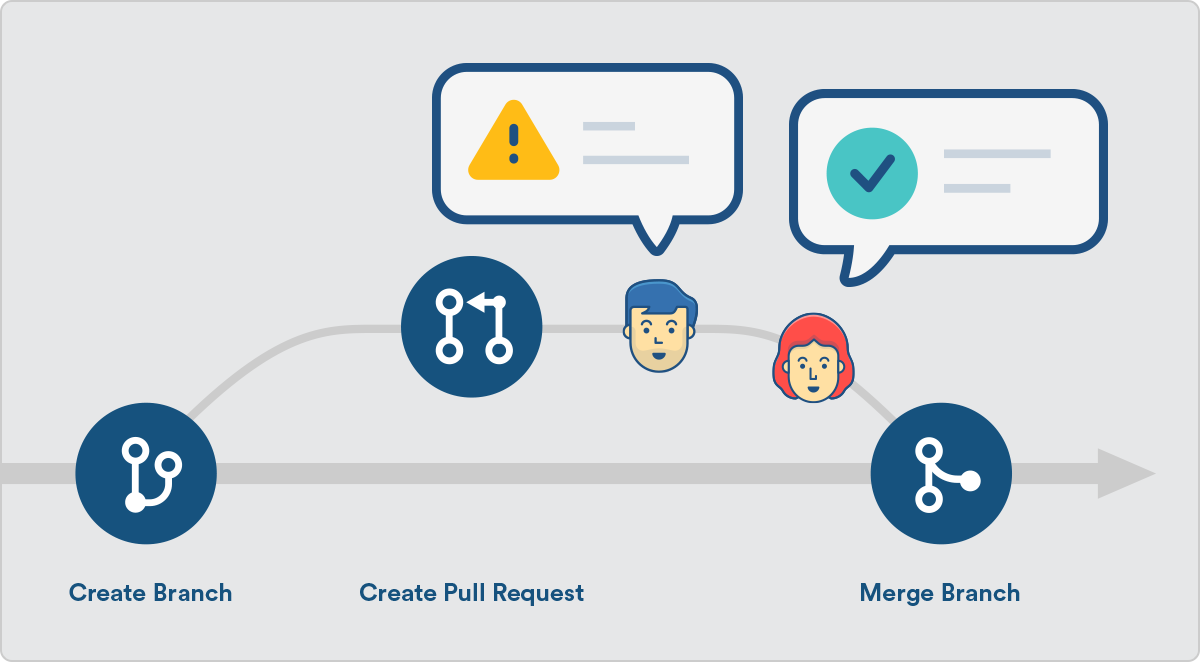
\includegraphics[width=0.6\textwidth]{./images/git_pr.png}
        \caption{Pull request. Imagen obtenida de 
        \href{https://unr-omics.readthedocs.io/en/latest/git_lesson.html}{https://unr-omics.readthedocs.io/}}
    \end{figure}
\end{frame}


\end{document}